\begin{center}
\Huge
Monotonisætningen og monotoniforhold
\end{center}
\section*{Monotonisætningen}
\stepcounter{section}
Hvis en funktion aftager efter et toppunkt og funktionen ikke har flere ekstremumspunkter til højre for dette toppunkt, så virker det intuitivt at funktionen bliver ved med at aftage efter toppunktet. Dette gælder også tilsvarende for voksende funktioner og minima. Vi har en sætning, der præciserer denne idé for differentiable funktioner. Denne kalder vi for monotonisætningen. 
\begin{setn}[Monotonisætningen]
Lad $f$ være differentiabel på et interval $[a,b]$. Så gælder der følgende:
\begin{enumerate}[label=\roman*)]
\item Hvis $f'(x)>0$ for alle $x$ i intervallet $[a,b]$, så vil $f$ være voksende på $[a,b]$.
\item Hvis $f'(x)<0$ for alle $x$ i intervallet $[a,b]$, så vil $f$ være aftagende på $[a,b]$. 
\item Hvis $f'(x)=0$ for alle $x$ i intervallet $[a,b]$, så er $f$ konstant på $[a,b]$.
\end{enumerate}
\end{setn}
Det er ikke svært at bevise monotonisætningen, men det er derimod en smule omfattende. 
Til at bevise monotonisætningen bruges typisk et helt centralt bevis i differentialregningen. Middelværdisætningen. Den lyder som følgende.
\begin{setn}[Middelværdisætningen]
	For en differentiabel funktion $f: [a,b] \to \mathbb{R}$
	findes der et indre punkt i definitionsmængden $c \in ]a,b[$, så
	\begin{align*}
		f'(c) = \frac{f(b)-f(a)}{b-a}.
	\end{align*}
\end{setn}
Dette betyder, at sekanthældningen for en sekant mellem to punkter for en differentiabel funktion $f$ altid er lig med differentialkvotienten i et punkt på grafen mellem de to punkter. Dette virker ganske intuitivt, og måske også en smule banalt, men det er et ganske vigtigt resultat.
På Figur \ref{fig:middel} ses en illustration af middelværdisætningen. 

\begin{figure}[H]
	\centering
	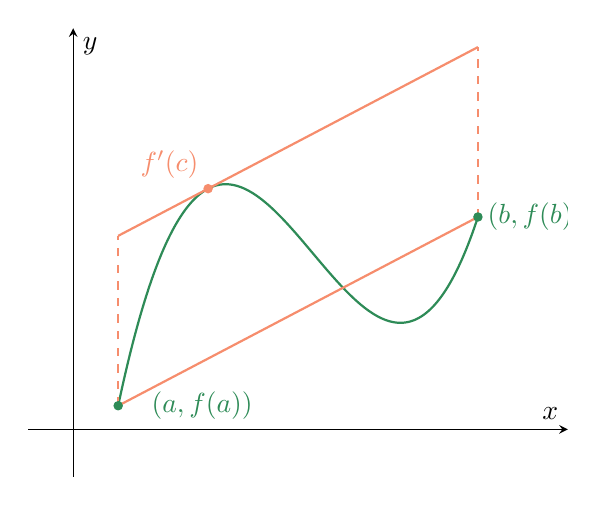
\begin{tikzpicture}
	\begin{axis}[
		axis lines = center, 
		xmin = -1, xmax = 11,
		ymin = -1, ymax = 8.5,
		xlabel = $x$, ylabel = $y$,
		ticks = none,
		]
		\addplot[samples = 400, domain = 1:9, thick, color = SeaGreen] {0.1*(x-4)^3 - 0.4*(x-4)^2 - 0.6*(x-4) + 5};
		\draw[color = Melon, thick] (axis cs: 1, 0.5) -- (axis cs: 9, 4.5);
		\draw[color = Melon, thick] (axis cs: 1, 0.5+3.6) -- (axis cs: 9, 4.5+3.6); 
		\draw[color = Melon, thick, dashed] (axis cs: 1, 0.5) -- (axis cs: 1, 0.5 + 3.6);
		\draw[color = Melon, thick, dashed] (axis cs: 9, 4.5) -- (axis cs: 9, 4.5 + 3.6);
		\filldraw[color = SeaGreen] (axis cs: 1, 0.5) circle (1.5pt) node[anchor = west, xshift = 3mm] {$(a,f(a))$};
		\filldraw[color = SeaGreen] (axis cs: 9, 4.5) circle (1.5pt) node[anchor = west] {$(b,f(b))$};
		\filldraw[color = Melon] (axis cs: 3, 5.1) circle (1.5pt) node[anchor = south east] {$f'(c)$};
	\end{axis}
	\end{tikzpicture}
	\caption{Sekant mellem $(a,f(a))$ og $(b,f(b))$ samt tangent i punktet $(c,f(c))$ begge med hældningen $f'(c)$, der illustrerer middelværdisætningen.}
	\label{fig:middel}
\end{figure}

Vi skal hovedsagligt bruge monotonisætningen til at bestemme monotoniforhold for differentiable funktioner. Vi arbejdede også med monotoniforhold i 1.g, men vi skal nu kunne bestemme monotoniforhold uden tegninger af grafer.
\newpage
\begin{exa}
Vi så i 1.g på en funktion, der mindede meget om funktionen $f$, der kan ses på Figur \ref{fig:monotoni}.
	\begin{figure}[H]
		\centering
		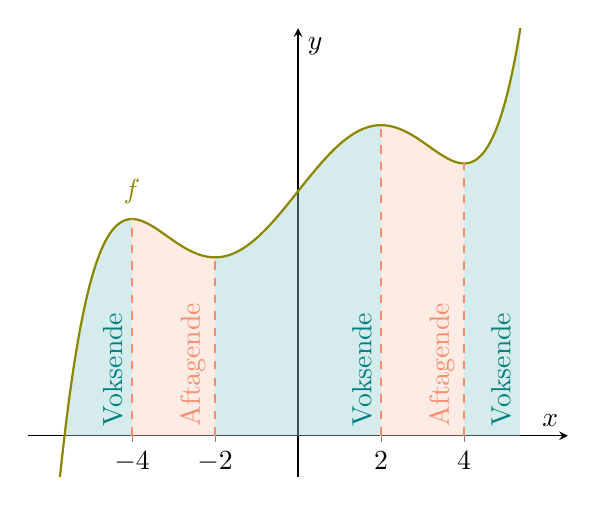
\begin{tikzpicture}
		\begin{axis}[
		axis lines = center,
		xmin = -6.5,xmax = 6.5,
		ymin = -50,ymax = 500,
		xlabel= $x$, ylabel = $y$,
		xtick = {-4,-2,2,4},
		ytick = {0},
		]	
			%voksende
			\fill[color = teal!40, variable = \x, domain = -5.625:-4,opacity = 0.4] (axis cs:-5.625,0) --
			 plot (axis cs: \x, 64*\x - 20/3*\x^3 + 1/5*\x^5 + 300) -- (axis cs: -4,0) -- cycle;
			%aftagende
			\fill[color = Melon!40, variable = \x, domain = -4:-2,opacity = 0.4] (axis cs:-4,0) --
			 plot (axis cs: \x, 64*\x - 20/3*\x^3 + 1/5*\x^5 + 300) -- (axis cs: -2,0) -- cycle;
			%voksende
			\fill[color = teal!40, variable = \x, domain = -2:2, opacity = 0.4] (axis cs:-2,0) --
			 plot (axis cs: \x, 64*\x - 20/3*\x^3 + 1/5*\x^5 + 300) -- (axis cs: 2,0) -- cycle;
			%aftagende
			\fill[color = Melon!40, variable = \x, domain = 2:4,opacity = 0.4] (axis cs:2,0) --
			 plot (axis cs: \x, 64*\x - 20/3*\x^3 + 1/5*\x^5 + 300) -- (axis cs: 4,0) -- cycle;
			%voksende
			\fill[color = teal!40, variable = \x, domain = 4:5.35,opacity = 0.4] (axis cs:4,0) --
			 plot (axis cs: \x, 64*\x - 20/3*\x^3 + 1/5*\x^5 + 300) -- (axis cs: 5.35,0) -- cycle;
			\addplot[color = olive, thick, samples = 500, domain = -6:6] {64*x - (20*x^3)/3 + 1/5*x^5 + 300};
 			\node[color = olive] at (axis cs: -4,300) {$f$};
 			\draw[color = Melon, dashed, thick] (axis cs:-4,0) -- (axis cs:-4,265.867);
 			\draw[color = Melon, dashed, thick] (axis cs:-2,0) -- (axis cs:-2,218.933);
 			\draw[color = Melon, dashed, thick] (axis cs:2,0) -- (axis cs:2,381.067);
 			\draw[color = Melon, dashed, thick] (axis cs:4,0) -- (axis cs:4,334.133);
			\node[color = teal, anchor = south west, rotate = 90] at (axis cs: -4,0) {Voksende};
			\node[color = Melon, anchor = south west, rotate = 90] at (axis cs: -2,0) {Aftagende};
			\node[color = teal, anchor = south west, rotate = 90] at (axis cs: 2,0) {Voksende};
			\node[color = Melon, anchor = south west, rotate = 90] at (axis cs: 4,0) {Aftagende};
			\node[color = teal, anchor = south west, rotate = 90] at (axis cs: 5.35,0) {Voksende};
		\end{axis}
		\end{tikzpicture}
		\caption{Graf for $f$ med monotone intervaller markeret.}
		\label{fig:monotoni}
	\end{figure}
	Vi kan nu opskrive monotoniforholdene for funktionen $f$.
	\begin{itemize}
		\item[$\cdot$] $f$ er voksende for $x \in ]-\infty,-4]$.
		\item[$\cdot$] $f$ er aftagende for $x \in [-4,-2]$.
		\item[$\cdot$] $f$ er voksende for $x \in [-2,2]$.
		\item[$\cdot$] $f$ er aftagende for $x \in [2,4]$.
		\item[$\cdot$] $f$ er voksende for $x \in [4,+\infty[$.
	\end{itemize}
	Vi kan også som sidste bruge foreningsmængden $\cup$ til at opskrive monotoniforholdene lidt mere kompakt.
	\begin{itemize}
		\item[$\cdot$] $f$ er voksende for $x \in ]-\infty,-4] \cup [-2,2] \cup [4,+\infty[$.
		\item[$\cdot$] $f$ er aftagende for $x \in [-4,-2] \cup [2,4]$.
	\end{itemize}
	Det er muligt at bestemme monotoniforholdene uden at bruge grafen. 
	Vi finder først ekstrema ved at differentiere og sætte lig 0 ved brug af Maple.
	\begin{align*}
		f'(x) = 64 - 20x^2+x^4 = 0
	\end{align*}
	Denne ligning løses med Maple, og vi får løsningerne $x = -4$, $x= -2$, $x = 2$ og $x = 4$. Disse er altså ekstrema 
	for $f$, hvilket vi også kan se på Figur \ref{fig:monotoni}.
	Vi skal nu bestemme hældningen for funktionen $f$ mellem funktionens ekstrema. Vi vælger derfor et tal før, mellem
	og efter alle ekstrema og bestemmer hældningen her.
	\begin{align*}
		&\textnormal{før }-4 & &f'(-5) = 189 > 0 \\
		&\textnormal{mellem }-4\textnormal{ og }-2 & &f'(-3) = -35 < 0 \\
		&\textnormal{mellem }-2\textnormal{ og }2 & &f'(0) = 64 > 0 \\
		&\textnormal{mellem }2\textnormal{ og }4 & &f'(3) = -35 < 0 \\
		&\textnormal{efter }4 & &f'(5) = 189 > 0 \\
	\end{align*}
	Disse hældninger passer til de monotoniforhold, vi allerede har opskrevet. 
\end{exa}
\begin{exa}
Vi skal også kunne bestemme monotoniforhold uden hjælpemidler. Vi ønsker derfor at bestemme monotoniforholdene for funktionen 
\begin{align*}
	f(x) = \frac{1}{3}x^3-\frac{1}{2}x^2-2x.
\end{align*}
For at finde monotoniforholdene for $f$ starter vi med at differentiere $f$ for at se, hvor $f$ har ekstremumspunkter. Vi finder derfor $f'(x) = x^2-x-2$ og sætter denne lig nul:
\begin{align*}
f'(x)=x^2-x-2 = 0,
\end{align*}
som har løsningerne $x=-1$ og $x=2$. Funktionen $f$ har derfor ekstremumspunkter i $x=-1$ og $x=2$. Vi bruger $f'$ til at afgøre, hvornår $f$ er voksende og aftagende ved at indsætte et tal på $x$ plads mellem $-1$ og $2$, et tal mindre end $-1$ og et tal større end $2$. Derfor får vi
\begin{align*}
f'(-2) = (-2)^2+2-2 = 4, 
\end{align*} 
og monotonisætningen siger derfor, at $f$ vokser på intervallet $]-\infty,-1]$. 
\begin{align*}
f'(0) = 0^2-0-2 = -2,
\end{align*}
og monotonisætningen siger derfor, at $f$ aftager på intervallet $[-1,2]$.
\[ 
f(3) = 3^2-3-2 = 9-5=4,
\]
og monotonisætningen siger derfor, at $f$ vokser på intervallet $[2,\infty[.$
For at være helt præcise opskriver vi monotoniforholdene:
\newpage
\begin{itemize}
	\item[$\cdot$] $f$ er voksende for $x \in ]-\infty,-1]$
	\item[$\cdot$] $f$ er aftagende for $x \in [-1,2]$
	\item[$\cdot$] $f$ er voksende for $x \in [2,\infty[$
\end{itemize}
Vi opskriver desuden en monotonilinje.
\begin{center}
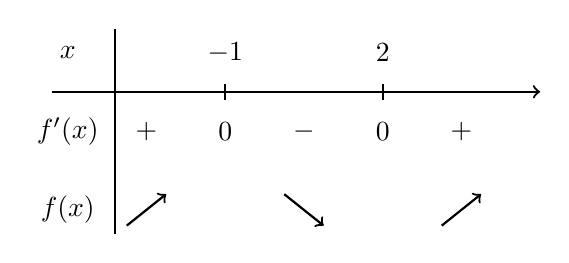
\begin{tikzpicture}
\node at (0,0) {$x$};
\node at (0,-1) {$f'(x)$};
\node at (0,-2) {$f(x)$};
\node at (2,0) {$-1$};
\node at (4,0) {$2$};
\node at (2,-1) {0};
\node at (4,-1) {0};
\node at (1,-1) {$+$};
\node at (3,-1) {$-$};
\node at (5,-1) {$+$};
\draw[->,thick] (-0.2,-0.5) to (6,-0.5);
\draw[thick] (2,-0.6) to (2,-0.4);
\draw[thick] (4,-0.6) to (4,-0.4);
\draw[thick] (0.6,0.3) to (0.6,-2.3);
\draw[->,thick] (0.75,-2.2) to (1.25,-1.8);
\draw[->,thick] (2+0.75,-1.8) to (2+1.25,-2.2);
\draw[->,thick] (4+0.75,-2.2) to (4+1.25,-1.8);
\end{tikzpicture}
\end{center}
\end{exa}

\subsection*{Opgave 1}
For en funktion $g$ gælder der, at $g'(x) = 0$ hvis og kun hvis $x = 2$ eller $x = 4$ samt at $g'(-4) = 1$, $g'(3) = 2$ og $g'(5) = -2$. Opskriv monotoniforholdene for $g$.

\subsection*{Opgave 2}
Bestem monotoniforholdene for følgende funktioner. Sørg også for at tegne funktionerne for at verificere dine monotoniforhold. 
\begin{align*}
&1) \ f(x) = x^2   &&2)\  f(x) = x^4 - 32x^2 + 10 \\
&3) \ f(x) = x^3 - 3x^2 - 9x -10 &&4)\ f(x) = x^3 \\
&5) \ f(x) = x^4-8x^2 &&6)\ f(x) = \ln(x) -\frac{1}{2}x^2 \\
&7) \ f(x) = \frac{2}{5}x^5-27x^2  &&8)\ f(x) =  \cos(x), \quad 0 \leq x \leq 4\pi
\end{align*}

\subsection*{Opgave 3}
Vi vil i denne opgave bevise monotonisætningen. Beviset for i) fremgår her, og så skal I selv bevise ii) og iii)
\begin{proof}
	Vi beviser i) og antager derfor, at $f'(x) > 0$ for alle $x \in [a,b]$.
	
	Vi vælger nu $x_1, x_2 \in ]a,b[$, så $x_2 > x_1$. Middelværdisætningen giver os nu et tal $c \in ]x_1,x_2[$, så
	\begin{align*}
		f'(c) = \frac{f(x_2)-f(x_1)}{x_2-x_1}.
	\end{align*}
	Vi ganger med $x_2 - x_1$ på begge sider af lighedstegnet og får
	\begin{align*}
		f'(c)(x_2 - x_1) = f(x_2) - f(x_1).
	\end{align*}
	Men da $f'(c) > 0$, og $x_2 - x_1 > 0$, så må $f'(c)(x_2 - x_1) > 0$, og derfor må $f(x_2) - f(x_1) > 0$, hvilket betyder at $f(x_2) > f(x_1)$, og derfor må $f$ altså være voksende på $[a,b]$. 
\end{proof}
\begin{enumerate}[label= \Roman*)]	
	\item Bevis del ii) i monotonisætningen.
	\item Bevis del iii) i monotonisætningen. 
\end{enumerate}

\subsection*{Opgave 4}
	Vi ønsker også at bevise middelværdisætningen. Dette gøres med Rolles sætning, der i virkeligheden er et specialtilfælde af middelværdisætningen, og som vi ikke beviser. 
	\begin{setn}[Rolles sætning]
		Hvis en differentiabel funktion $f: [a,b] \to \mathbb{R}$ opfylder, at $f(a) = f(b) = 0$, så findes der et 
		$c \in ]a,b[$, så
		\begin{align*}
				f'(c) = 0.
		\end{align*}
	\end{setn}
	Vi skal nu bevise middelværdisætningen. 
	\begin{enumerate}[label=\roman*)]
		\item Opskriv forskriften for linjen $l(x)$, der går gennem $(a,f(a))$ og $(b,f(b))$ på Figur \ref{fig:middel}. (Kald blot skæringen med $y$-aksen for $\beta$.)
		\item Opskriv $h(x) = f(x) - l(x)$ og argumentér for, at $h$ opfylder betingelserne i Rolles sætning. 
		\item Opskriv $h'(x)$ og dernæst $h'(c) = 0$.
		\item Argumentér for, at dette viser, at 
		\begin{align*}
			f'(c) = \frac{f(b) - f(a)}{b - a},
		\end{align*}
		og at beviset hermed er færdigt. 
	\end{enumerate}